\documentclass[fleqn,envcountsame,runningheads,10pt,a4paper]{llncs}

\usepackage[utf8]{inputenc}
\usepackage{enumerate}
\usepackage{verbatim}
\usepackage{moreverb}
\usepackage{subfigure}
\usepackage{graphicx}
\usepackage{amsmath}
\usepackage{amsfonts}
\usepackage{amssymb}
\usepackage{cite}
\usepackage{url}
\usepackage{hyperref}

\pagestyle{headings}

\begin{document}
\title{Razor: A Low-Power Pipeline Based on Circuit-Level Timing Speculation}
\titlerunning{Razor: A Low-Power Pipeline Based on Circuit-Level Timing Speculation}
\author{Nicolas Bonfante}
\authorrunning{Nicolas Bonfante}
\institute{Universität Passau}

\maketitle

\begin{abstract}
Due to many progress in circuit manufacturing and design (increasing of clock frequencies, decreasing of circuit size... ), the problem of power consumption has become an essential concern. Some mechanisms are currently used to reduce the circuit consumption but they are based on worst-case scenario that are rarely obtain in a real-life working. 

This paper will explain the principle and benefits of Razor : a low-power pipeline based on circuit-level timing speculation. The main idea is to tune the supply voltage during the circuit operation and come back to a correct state if the system detects an error.
\end{abstract}


\section{Introduction}
Nowadays, we have more and more powerful devices and we want more and more battery life. Moreover, our devices are now able to execute different tasks (reading video or music, taking photos, ...) that do not need the same voltage supply. Some tasks need more power to be executed successfully. To obtain better battery-life, electronic devices use Dynamic Voltage Scaling (DVS)\cite{Pering:1998}. The principle of DVS is to increase or decrease the voltage supply depending on the needs of the processor. The energy needed to ensure correct operation is correlated to many variabilities. These variabilities can be local (cross-coupling) or global (temperature, supply drop). The voltage needed is also heavily dependant on the data. The minimum possible voltage supply is called critical supply voltage. The technique described in this article is profitable for every chips and especially processors.

For now, the main principle of DVS is to estimate at design-time a conservative supply voltage (lowest supply voltage to ensure correct operation) using modelling and worst-case scenarii. This method uses margins and is therefore not optimal because the worst-case scenarii are very rarely obtain in real-life operation. The Razor DVS technique is based on dynamic detection and correction of speed path failures. The idea is to adjust the supply voltage by analysing the error-rate during circuit operation. As Razor is based on dynamic detection, it can handle both local and global variabilities and does not need voltage margins. A key feature of Razor is that operate at a sub-critical supply voltage is not disastrous. Only few instructions will fail because of too low voltage. But the others will output the correct result and use less energy. The idea is to balance the saving due to lowering the voltage and the loss due to error recovery.

Figure \ref{figure3} represents a version of Razor. The main flip-flop, part of the circuit without Razor, is the flip-flop that need error-detection. Each delay-critical flip-flop is augmented with a shadow latch. The main flip-flop is controlled by the main clock of the system whereas the shadow latch is controlled by a delayed clock. If the logic stage L1 is too slow with the current supply voltage, the data in the main flip-flop will not be correct. But if the operating voltage is constrained such that the worst-case delay is consistent with the setup-time of the shadow latch, the correct value will be caught by the shadow latch. So by comparing the value of the main flip-flop and of the shadow latch, it is possible to detect an error. 

This paper is organised as follows. The section 2 is a discussion on how Razor detect and correct errors. Circuit-level requirements, error recovery mechanism and supply voltage control will be presented. In section 3, the error rate will be analysed. The section 4 will talked about experimental evaluation. Finally, the conclusion will be drawn in section 5. 

\section{Detection/correction mechanisms}
Razor combines architectural and circuit-level techniques for efficient error detection and correction. Each flip-flops is augmented with a shadow latch, controlled by a delayed clock. Figure \ref{figure2} represents the behaviour of a razor cell.
\begin{figure}[!h]
    \centering
   \centerline{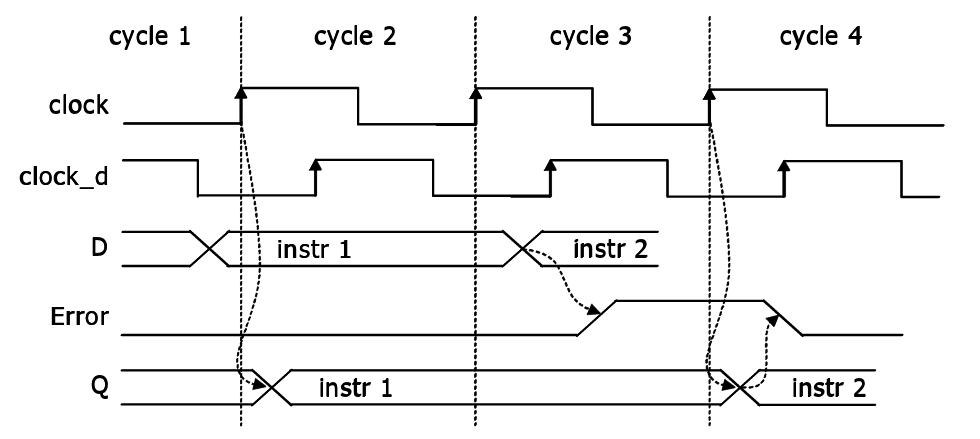
\includegraphics[scale=0.3]{./img/figure2.png}}
   \caption{\label{figure2}Error recovery chronograms\cite{Barthou:1998}}
\end{figure}
At cycle 1, the logic bloc L1 meets the setup time of the main flip-flop therefore both shadow latch and main flip-flop will get the correct data. At cycle 2, L1 exceeds the delay because of the insufficient voltage supply. The main flip-flop will then still contains the old data. But the shadow latch, due to the delayed clock, get the correct result at cycle 3. By comparing the values stored in the main flip-flop and in the shadow latch, it is possible to detect an error. When the error is detected, the Error\_L bit is set to one. At cycle 4, the correct value is load into the main flip-flop from the shadow latch. The pipeline is then ready to re-execute failed instructions. In theory, to recover from error, Razor only need only one extra cycle. 

If a logic bloc L1 fail, the data in L2 is wrong and must be remove from the pipeline using one of the methods described in sub-section~\ref{ERM}. One of the main feature of Razor is that error recovery does not need the re-computation of the failed instruction, because the lowest voltage supply is design such that the value in the shadow latch is always correct. Therefore we only need one extra cycle to put the correct value in the failed pipeline. This property guarantees the forward progress : if an instruction fails, it can not fail again because the correct value is in the shadow latch. 

The razor extra circuit must be designed such that the power and delay overhead is minimised. Also, the delayed clock introduces a new short-path constraint in the design. Finally, allowing the setup time of the main flip flop to be exceeded can create meta-stability problems. All these circuit-level problems will be discussed in sub-section~\ref{CLR}.

The goal of Razor is to manage the voltage supply such that it is always optimal. Therefore a mechanism to tune the supply voltage is needed. The sub-section~\ref{SVC} will discuss about the technique used to control voltage according to the error base rate.

\subsection{Circuit-level requirements}
\label{CLR}
A requirement for an efficient DVS is that during error-free operation, the delay and power overhead due to the detection part must be minimal. Otherwise the gain due to the voltage scaling will be lost. Moreover, the cost of error-recovery should be as small as possible to allow efficient operation when some errors occur. For instance, to reduce the cost of Razor operation, the delayed clock can be generated locally. If we want a delayed clock by half the main clock cycle, we can just invert locally the main clock to obtain the delayed one. It is also important to notice that many flip-flops do not need a Razor mechanism  because they can operate correctly under a sub-critical voltage. For example, in an Alpha processor only 192 out of 2048 flip-flops actually required a Razor mechanism.

Allowing the fact that the logic bloc L1 finishes his task after the main clock edge can give rise to meta-stability problems in the main flip-flops. If the main flip-flop input varies at the same time as its clock, the flip-flop may be not able to resolve the value of the input because the input is in a transient state. This problem can not occur in the shadow latch because this part of the circuit is designed such that in the worst-case scenario, the setup-time of the shadow latch is always met. If the main flip-flop is in a meta-stable state, it is impossible to determine if the system is in error or not. This is the reason why a circuit (called Local Meta-detector in figure \ref{figure3}) to detect meta-stability has been introduced. In case of meta-stability issues, the value is restored from the shadow latch like in case of error.

It can happened that the error signal itself has meta-stability problems. The so called Global Meta-detector in figure \ref{figure3} handle such a case. If a meta-stability is detected in the error signal, a panic signal is generated and the whole pipeline is restored. 
\begin{figure}[!h]
    \centering
   \centerline{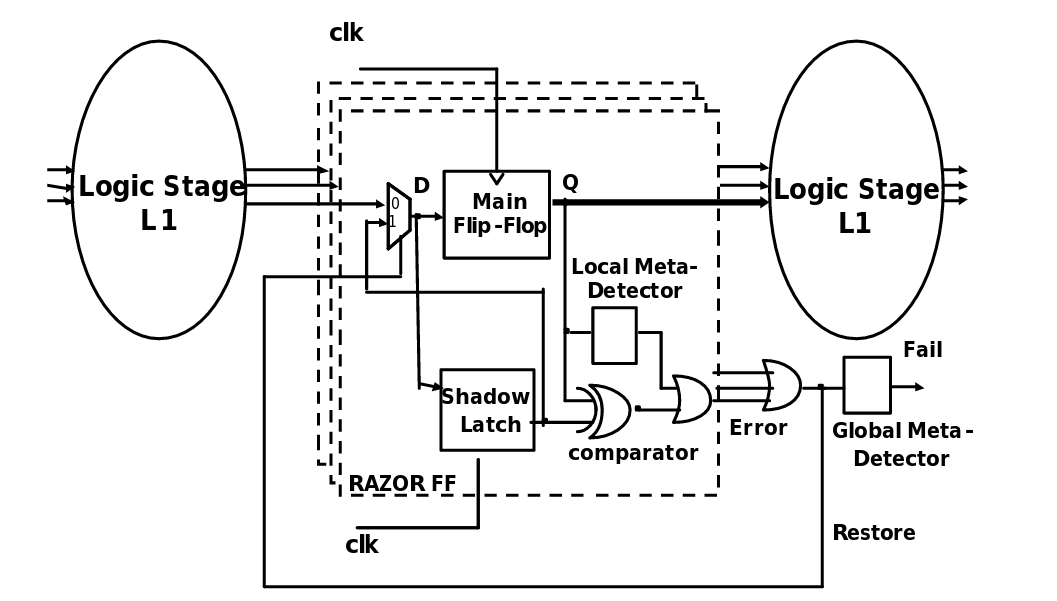
\includegraphics[scale=0.25]{./img/figure3.png}}
   \caption{\label{figure3}Reduced overhead Razor circuit\cite{Barthou:1998}}
\end{figure}

\subsection{Error recovery mechanisms}
\label{ERM}
The error recovery mechanisms is the piece of hardware that guarantees that, when an error occurs, register and memory are not corrupted with incorrect values. Two methods are described in the paper. The first one is called clock gating which is slow but simple. The second one is based on counterflow pipelining and is supposed to be more scalable.

\subsubsection{Clock gating}
The idea of clock gating is that, if errors occur, the whole pipeline is stop and logic blocs where the error occur recompute theirs values with the value in their shadow latch. Since the logic blocs recompute their result with the value in the shadow latch, any number of errors can be recovered in only one cycle. The forward progress is guaranteed because the value in the shadow latch is, by design, always correct. The worst-case scenario happen if all stages produce an error at each cycle. The speed will be half the speed of an error-free pipeline. 
Figure \ref{figure4} represents a pipeline where an error during EX instruction happen at 4th cycle. The error is caught at cycle 5, but the MEM stage is in the middle of computing with the wrong value. So we stop the pipeline at cycle 6 so that MEM stage can recompute his output with the value in the shadow-latch. To avoid wrong values to be used by the circuit after our pipeline (in this case, the value to be stored in the main memory), it is important to add another stage to stabilise (ST stage) the value, i.e wait 1 cycle to be sure that the value is correct. 
\begin{figure}[!h]
    \centering
   \centerline{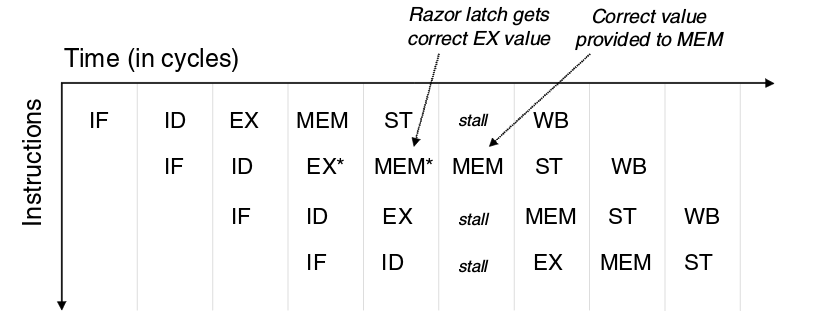
\includegraphics[scale=0.3]{./img/figure4.png}}
   \caption{\label{figure4}Clock gating recovery example\cite{Barthou:1998}}
\end{figure}

\subsubsection{Counterflow pipelining}
The main problem of the previous method is that the impact in the circuit is too significant. The cycle time must be long enough so that any stage in the pipeline can deliver a clock gating signal to the others flip-flops. The method described in this section is based on counterflow pipelining techniques\cite{Molnar:1994}. The impact in the circuit is small but in return the recovery of an error take more cycles. 
To explain the principle of this method, let use an example. Figure \ref{figure5} represents a pipeline in error at the same stage as before : EX stage at cycle 4. This error is detected at cycle 5, then a bubble is generated out of the MEM stage and the flush train is initialise. Then at cycle 6,7,8, the EX, ID and IF stage are flushed. 
\begin{figure}[!h]
    \centering
   \centerline{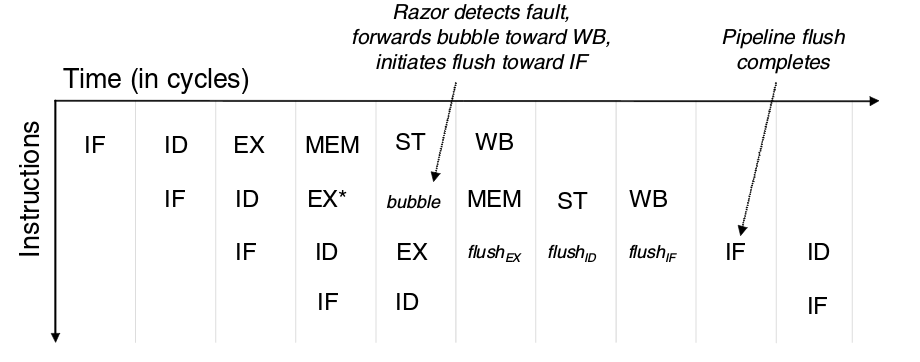
\includegraphics[scale=0.3]{./img/figure5.png}}
   \caption{\label{figure5}Counter-flow pipe-lining recovery example\cite{Barthou:1998}}
\end{figure}

\subsubsection{Requirements}
A recovery mechanism need to be resilient to error and must not fail under worst-case operations conditions (e.g., temperature, low voltage). For the recovery mechanism, a conservative approach is taken at design so that it is always fully functional. 

\subsection{Supply voltage control}
\label{SVC}
A lot of parameters can influence the voltage needed to operate with an acceptable error-rate. It depends on the temperature and can also vary with the processing demands (data and instruction dependant). It is desirable to have a voltage control system (VCS) into the design to optimise energy conservation. The role of the VCS is to manage the supply voltage based on the error-rate. The error rate is a good indicator to decide whether the voltage supply must be changed. If it is too low, the voltage supply can be lowered because this means that the circuit operate more or less without errors. In the other hand, if the error rate is too high, this means that too many errors occur and that the benefit of Razor will be lost due to recovery overhead.

In Razor, the VCS try to maintain a fixed error-rate called $E_{ref}$. At regular intervals, the real-time error rate $E_{sample}$ is measured. The system compare both value ($E_{diff} = E_{ref} - E_{sample}$). The magnitude of $E_{diff}$ indicates the degree to which the system is out of tune and the sign indicates if the VCS must lower or increase the voltage supply. We can see on the voltage Control Function bloc on figure \ref{figure6} that there is a panic input. In case of panic, the voltage supply in automatically increase, no matter the value of $E_{diff}$. 

\section{Error rate analysis}
In a first phase, the benefits of Razor were gauged by analysing the error rate. To do that, a 18x18bits multiplier was implemented within a FPGA. A 64bits Kogge-Stone adder was also implemented and analyse with SPICE.
\subsubsection{FPGA-based analysis}
The error-rate for the multiplier was analysed under different voltage and temperature. The results of the figure \ref{figure7} show the error-rate at 90MHz and at 27$\°$. 3 points are defined on this plot. The zero-margin point is the lowest voltage at which the circuit operate error-free. The safety-margin point is the point at which the circuit operates correctly in 90\% of the baseline clock period at 27$\°$. The environmental-margin point is the safety-margin for 85$\°$. Such a circuit that operates with an error rate of 1\% would save up to 22\% compare to the zero-margin point. An energy-save of this magnitude is considerable.
\begin{figure}[!h]
    \centering
   \centerline{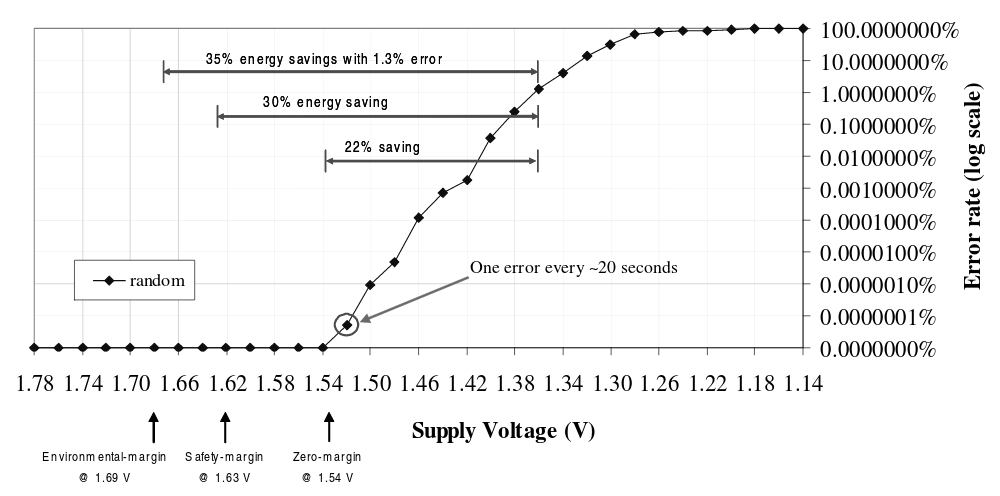
\includegraphics[scale=0.35]{./img/figure7.png}}
   \caption{\label{figure7}Measured error rates for 18x18 multipliers at 90MHz and 27$\°$C\cite{Barthou:1998}}
\end{figure}

\subsubsection{SPICE-based analysis}
To understand the nature of circuit-timing error, a Kogge-Stone adder has been simulated using SPICE. The results in figure \ref{figure8} show that the extreme points and gain are heavily linked to the data the circuit operate on. 
\begin{figure}[!h]
    \centering
   \centerline{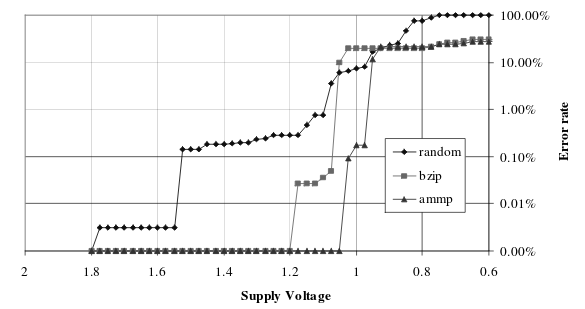
\includegraphics[scale=0.5]{./img/figure8.png}}
   \caption{\label{figure8}Simulated error rate for an adder at 870MHz and 27$\°$C\cite{Barthou:1998}}
\end{figure}

\section{Experimental evaluation}
To evaluate Razor, a 64-bit Alpha processor was augmented with Razor latches. This processor has a simple pipeline : IF, ID, EX, MEM/WB. In-depth analysis showed that only the ID and EX stages need Razor augmentation. Out of the 2048 flip-flops in the original design, only 192 were Razor-augmented. Power analysis was performed using gate level power simulation and SPICE. SPICE is an open-source circuit simulator. 

11 programs from the SPEC2000 benchmarks were compiled for this Alpha processor. The results of this benchmark can be found in table \ref{table1}. This table lists the energy reduction and IPC reduction. The energy saving only takes into account the data-dependent delay because the energy is compared to the zero-margin point. Even if the energy reduction is huge, the IPC is not that much affected.
\begin{table}[t]
\centering
    \caption{\label{table1} Simulated DVS energy saving}
    \begin{tabular}{|l|l|l|}
        \hline
        Program & \%Energy reduced & \%IPC reduced \\ \hline
        bzip    & 54.5            & 4.13         \\ 
        crafty  & 54.8            & 1.78         \\ 
        eon     & 30.4            & 0.78         \\ 
        gap     & 12.9            & 2.14         \\ 
        gcc     & 31.3            & 5.88         \\ 
        gzip    & 44.6            & 1.27         \\ 
        mcf     & 36.9            & 0.47         \\ 
        parser  & 53.0            & 1.94         \\ 
        twolf   & 20.4            & 0.06         \\ 
        vortex  & 49.1            & 1.07         \\ 
        vpr     & 63.6            & 1.66         \\ 
        Average & 41.0            & ~            \\
        \hline
    \end{tabular}
\end{table}

\section{Conclusion}
Razor is a dynamic voltage scaling technology that allow error in the pipeline. The key principle of Razor is the fact that he operates in-situ so there is no need for margins. Compare to others DVS systems, Razor is the only one who is able to get rid of the data, process, environmental and safety margins. A latch, controlled by a delayed clock, is added to every unsafe flip-flop so that the latch always catch the correct value even if the main flip-flop miss the clock edge. The design of such a mechanism is not problem-free. The energy cost of the added circuit must be as small as possible and it must be reliable. Simulations show that a Razor adder operate with 41\% less energy while having only a small impact on the IPC. 
\bibliographystyle{splncs}
\bibliography{literature}
\end{document}
